\chapter{Espaço Aéreo, Tráfego e Equipe de Vôo}\label{cha:airspace}
Um arquivo de dados de uso especial de espaço aéreo (Special Use Airspace - SUA) pode ser baixado para o XCSoar e usado tanto para mostrar as regiões de espaço aéreo e detectar quando a aeronave entra e deixa estas regiões.

Dois arquivos podem ser encontrados de espaço aéreo nos ajustes das configurações.  O primeiro é usado para banco de dados primários SUA e o segundo é para ser utilizado com as alterações de espaços aéreos, como áreas definidas por NOTAMs.

É de responsabilidade do piloto se assegurar que o banco de dados USA está atualizado.

Através de um dispositivo FLARM conectado, o computador pode também mostrar a relação entre o tráfego aéreo equipados também com FLARM e ameaças de obstáculos.

O código de time permite aos pilotos trocarem informações sobre suas informações de posições através de rádio, codificadas e decodificadas pelo computador.


\section{Mostrador de espaço aéreo}

As regiões locais de uso especial do espaço aéreo são mostradas no mapa como áreas sombreadas com bordas finas.  As cores e padrões das áreas são específicas para categorias diferentes de espaço aéreo e podem ser configuradas pelo usuário.  Dependendo dos ajustes, o usuário pode escolher mostrar todos os espaços aéreos, somente espaços aéreos abaixo de certa altitude, somente espaços aéreos com uma separação de altura específica ou somente espaços aéreos abaixo da aeronave.
\sketch{figures/airspace.png}

Os padrões usados para mostrar as áreas de espaço aéreo incluem opaco, transparente (vazia) e vários padrões sombreados e pontilhados.  Os padrões não opacos são praticamente transparentes respeitando a topografia do terreno sobrepondo o espaço aéreo.  Porém, quando esta sobreposição aparece, todas as bordas são visíveis.  Mesmo quando os padrões de espaço aéreo não são mutualmente transparentes, todas as bordas dos espaços aéreos são mostradas no topo das áreas do espaço aéreo.
A tela e os alertas de espaço aéreo podem ser individualmente ligados ou desligados pelo usuário, como descrito na seção
~\ref{sec:airspace-filter}.

O padrão de cores dos espaços aéreos classes C, D, E e F são conforme as cartas ICAO. 


\subsection*{Eventos de Invasão}

Três tipos de eventos são detectados pelo XCSoar com relação ao SUA:
\begin{description}
\item[Invasão prevista] este evento é detectado quando a aeronave pode estar no caminho que irá resultar na entrada de espaço aéreo em determinado tempo no futur.  O tempo pode ser ajustado nas configurações “tempo de alerta”.

O uso de uma trilha longa nestes cálculos significa que o sistema pode prever invasões mesmo quando estiver na deriva do vento quando estiver girando termais.


%{\it DIAGRAM SHOWING DETECTION OF PREDICTED INCUSION WHEN CIRCLING AND
%  CRUISING}

\item[Entrando] este evento ocorre quando a aeronave entra em uma região de espaço aéreo.
\item[Saindo] este evento ocorre quando a aeronave deixa a região de espaço aéreo.
\end{description}
Em todos os casos, a divisa da região é definida pelas altitudes mínima e máxima para os níveis de vôo, especificadas no arquivo de espaço aéreo.

Os alertas de espaço aéreo continuarão mesmo que a área invadida estiver fora da tela.

Mesmo quando uma fonte de altitude barométrica está conectada, é usada preferencialmente a altitude do GPS para detectar a invasão do espaço aéreo.  Isto faz o sistema operar conforme as convenções de ter o espaço aéreo violado baseado na altitude QNH ajustada.



\section{Alertas de espaço aéreo }

O conceito de alertas de espaço aéreo é graduado em níveis:
\begin{description}
\item[Nenhum] aeronave fora e distante do espaço aéreo.
\item[\colorbox{AirspaceYellow}{PERTO}] a aeronave está prevista a entrar e está perto do espaço aéreo.
\item[\colorbox{AirspaceRed}{DENTRO}] a aeronave está dentro do espaço aéreo.
\end{description}

A todo instante, o XCSoar monitora a aeronave relativa ao espaço aéreo e mantém níveis de alertas para cada posição.  Os alertas de espaço aéreo são filtrados de acordo com as preferências, mas algumas categorias de espaço aéreo podem ter sido desativadas.  
\sketch{figures/airspacewarning.png}
TA sequência de eventos quando se invade um espaço aéreo resulta em dois tipos de alertas: quando perto (nível 1) e quando dentro (nível 2).

Toda vez que o nível de alerta aumenta (acima do nível 0) para qualquer espaço aéreo, a janela de alerta aparece, acompanhada de um bip do sistema para o Altair no PDA.  Quando não houver mais regiões de espaço aéreo com níveis abaixo de 0, a janela é fechada automaticamente. 


\subsection*{Janela de alerta de espaço aéreo}

A janela de alerta de espaço aéreo contém uma lista de até 4 alertas individuais.  O estado da aeronave tem cor vermelha se está dentro da área e amarelo se está perto.  Se o alerta for reconhecido, o texto é acinzentado.

Each list item occupies two rows, and includes the following details:\\
\verb+<NOME e Classe>               <TOP>   <Posição>+
\verb+<Tempo e distância> <BASE>+

The values in the list are continuously updated. 
Veja exemplo abaixo:\\
\verb+Bern TMA Class D                FL100     +\colorbox{AirspaceYellow}{near}
\verb+35 sec horizontal dist 1300     1750m+

Significa que a aeronave está a 1300m separada horizontalmente do espaço aéreo Classe D `Bern TMA', com a base em 1750m e teto a FL100.
Outro exemplo:\\
\verb+Bern CTRgld Class C             1350m     +\colorbox{AirspaceRed}{inside}
\verb+                                SFC+

Significa que a aeronave está dentro de espaço aéreo Classe C `Bern CTRgld', com base na altitude do terreno e teto em 1350m.

Se houver alertas de espaço aéreo, toda vez a janela de alerta de espaço aéreo será mostrada para você ver os detalhes somente tocando o alerta. (para Altair: selecionando e teclando ENTER).

\subsection*{Reconhecimento de alertas de espaço aéreo }

Quando uma janela de alerta está visível e um alerta de espaço aéreo está ativo, é possível fechar a janela de alerta sem reconhecer o alerta.  Dependendo do hardware usado, você deve pressionar ESC (no PC ou Altair) ou o botão “FECHAR”.

Quando um ou mais alertas forem visíveis na janela de alerta de espaço aéreo, o alerta pode ser reconhecido pressionando-se um dos botões da caixa janela.  Se a lista conter mais do que um alerta de espaço aéreo, pode ser usado o botão rotativo no Altair (ou o cursor no PDA) para fazer o reconhecimento de um alerta.

O significado dos botões de reconhecimento são:

\begin{description}
\item[Rec Espaço]  reconhecimento de todos os níveis de alertas e futuros, desta região de espaço aéreo específica enquanto a aeronave estiver a 2,5km de separação horizontal e 500m de separação vertical (tecla F5 no Altair).
\item[Rec Dia]  reconhecimento de todos os níveis de alerta e futuros desta região de espaço aéreo especifica para o restante do vôo (até que o Altair/XCSoar for reiniciado).  (Tecla F6 no Altair). 
\item[Fechar]  fechar a janela de alerta de espaço aéreo sem reconhecimento do espaço aéreo.  A janela se abrirá automaticamente se o nível de alerta do espaço aéreo aumentar.  (Tecla F7 no Altair).
  The dialogue will re-open automatically if the airspace warning level increases.
\end{description}

Note que nem todos os botões de reconhecimento podem estar visíveis para todos os níveis de alerta.  Particularmente, dentro da SUA, você não tem opção de fazer o reconhecimento do alerta (Rec Alerta), sendo que neste ponto nenhum alerta iminente de invasão de espaço aéreo será ativado, pois foi constatado que você já está dentro deste espaço aéreo.

As orientações para usar esta janela são:
\begin{itemize}
\item  não faça o reconhecimento do alerta a menos que seja sua intenção ou se você quer evitar o espaço aéreo.
\item O bip de alerta somente ocorre quando o nível de alerta aumenta.
\item O sistema de alerta foi projetado para permitir girar perto de espaços aéreos sem irritar o piloto com alertas estranhos.
\end{itemize}

Quando um alerta de espaço aéreo é reconhecido, a região desenhada na tela fica sem o padrão de cor.

Quando a aeronave é prevista para entrar em área SUA, ou realmente entra nesta área, o alerta é aumentado, apresentado com um alerta audível e uma mensagem descrevendo o tipo de alerta de espaço aéreo e alguns detalhes (incluindo classe do espaço aéreo, altitudes de base e teto ou nível de vôo).

O reconhecimento dos alertas irá se repetir após um certo tempo especificado nos ajustes de configurações “Tempo de Reconhecimento”.

Os reconhecimentos de alertas de espaço aéreo se aplicam a regiões individuais da SUA.  Se, por exemplo, a aeronave invade o espaço aéreo A e o piloto reconhece o alerta, e após alguns momentos é prevista sua entrada no espaço aéreo B, o alerta de espaço aéreo SUA de região B será aumentado.


\tip Se você deseja reconhecer os alertas de espaço aéreo e não quer que se repitam, ajuste um grande valor para a configuração “Tempo de reconhecimento”.

Os alertas de espaço aéreo e a trilha futura estimada são automaticamente limpos quando a posição da aeronave é limpa do espaço aéreo.

Simultaneamente, os alertas de espaço aéreo podem ocorrer se a aeronave (ou sua trilha futura) entrar em regiões de múltiplos espaços aéreos.  



\section{Consulta a espaço aéreo e detalhes}

Para dispositivos com tela de toque ou mouse, quando uma área de espaço aéreo é visível no mapa, pode ser consultada tocando a região do mapa.  O item listado do mapa irá aparecer e fornecer uma visão geral dos waypoints, espaços aéreos, etc., abaixo da ponta do dedo ou mouse.  As áreas SUA listadas tem detalhes similares aos fornecidos quando um nível de alerta é aumentado.  A consulta mostra todas as áreas de espaço aéreo quando houver espaço aéreo sobrepostos na área consultada.  
\sketch{figures/airspace_mapelements.png}
Selecionando SUA na lista e teclando  \button{Details} ou apertando a tecla ENTER, mostra todos os detalhes do espaço aéreo.

\tip Para usuários Altair: este tipo de consulta de detalhes do espaço aéreo também pode ser acessado através do modo panorâmico.  Mova o cursor até a localização desejada e clique no botão \button{Oque aqui?}.  A lista do item do mapa aparecerá e lhe mostrará os detalhes sob a posição do cursor.

%% To put at another place
%Through the button menus is the same map query available.
%The `What's here?' query brings up a map element list including the the nearest 
%airspace region. 
%\begin{quote}
%\bmenu{Info}\blink\bmenu{What's here?}
%\end{quote}

%% Probably wrong and outdated
%If the glider is outside the airspace, it also describes the distance
%and bearing to the nearest point on the airspace perimeter to the
%glider.  If the glider is inside the airspace, it also describes the
%distance and bearing to the nearest exit.

\subsection*{Janela de filtro de espaço aéreo}\label{sec:airspace-filter}

A janela de filtro de espaço aéreo permite que se ative ou desative os alertas para cada classe de espaço aéreo.  

Pode ser acessada:
\begin{itemize}
\item Através do menu principal   \bmenug{Config 3}\blink\bmenug{Espaço Aéreo}.
\item Ou através da página de configuração do sistema para espaço aéreo, tecle no botão \button{Filtro}.
\end{itemize}

\sketch{figures/airspacefilter.png}
Ou através da página de configuração do sistema para espaço aéreo, tecle no botão

\subsection*{Janela de seleção de espaço aéreo}

Teclando no botão Lookup abre a janela de seleção do espaço aéreo.  Esta função é similar à procura de waypoints e permite procurar por nome, distância, direção e tipo (classe).
\sketch{figures/airspacelookup.png}

Uma vez que o espaço aéreo foi localizado, você deve reconhecê-lo durante este dia.  Através da janela de gerenciamento de espaço aéreo possível reativá-lo novamente.


\section{Janela de Análise}

A janela de análise contém uma página que mostra um corte (seção) do espaço aéreo.
\menulabel{\bmenug{Info 1}\blink\bmenug{Analysis}}

TA tela mostra ao longo da direção horizontal, a distância da aeronave até 50km na direção da trilha da aeronave.  Na direção vertical está a altitude.  A altitude da aeronave é indicada por uma seta branca.  Esta página é útil para visualizar as camadas mais complexas do espaço aéreo.

\begin{center}
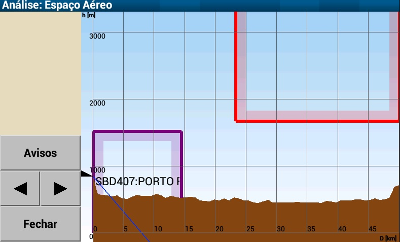
\includegraphics[angle=0,width=0.8\linewidth,keepaspectratio='true']{figures/analysis-airspace.png}
\end{center}

O botão de alerta abre a janela de alerta de espaço aéreo se estiver perto do espaço aéreo.


\section{Tráfego FLARM }

Se conectado a um dispositivo FLARM, o tráfego FLARM é mostrado na área do mapa.  Cada aeronave FLARM recebida é desenhada como um disco sombreado vermelho.

\warning Não use o XCSoar para evitar colisões, os dispositivos sonoros FLARM são mais recomendáveis para ajudar o piloto a ficar atento ao tráfego.

Observe que, se somente uma aeronave está girando, o nível de zoom normal é tal que o tráfego FLARM não será facilmente distinguido.  Quando somente uma aeronave estiver girando, o nível de zoom deve ser apropriado, mas a mudança constante de direção e a latência típica dos PDAs não ajudam muito a localizar o tráfego na tela do mapa.


\subsection*{Visualização do mapa FLARM}

Os alvos FLARM no mapa são desenhados como uma seta vermelha para indicar a direção que o alvo FLARM está indo, bem como o risco de colisão.  \config{flarm-on-map} Observe que as pontas destas setas são orientadas de acordo com a orientação da tela.  Por exemplo, se a orientação está ‘Rota acima’, a seta irá mostrar a direção da aeronave alvo com relação a sua aeronave.  Se a orientação da tela está ‘Norte acima’, a seta irá mostrar a rota absoluta da direção de aeronave alvo. 
\sketch{figures/flarmmap.png}

O registro da aeronave FLARM ou o nome do piloto pode ser visível no mapa através da localização da identificação ICAO da aeronave de tráfego FLARM no arquivo.  Veja seção ~\ref{sec:flarm-ident-file} para mais detalhes do formato do arquivo.  As aeronaves com privacidade FLARM não terão qualquer identificação mostrada. 

\subsection*{Radar FLARM}

Quando um alarme de trafego FLARM é recebido, o XCSoar mostra um pequeno radar com o tráfego FLARM da perspectiva da aeronave.  O tráfego FLARM é mostrado em estilo idêntico, com exceção de que o tráfego de ameaça é enfatizado com um ou dois círculos em volta do ícone de seta.  A visualização usada para este pequeno radar pode ser configurada.\config{flarmradar-place}.

O mostrador FLARM é orientado ‘rota acima’ e um pequeno ícone de planador é mostrado bem como sua orientação.  A escala do mostrador é linear até o máximo de 2.000 metros de distância.  Ao fundo há dois anéis: o primeiro tem raio de 1.000 metros e o segundo com 2.000 metros.  O tráfego mais distante do que 2.000 metros é mostrado no anel de 2.000 metros.
\sketch{figures/flarmrose.png}

Todo o mostrador FLARM mostra o tráfego FLARM em cores, de acordo com o nível de ameaça ou time e janela de estado.  O tráfego é colorido conforme abaixo:
\begin{itemize}
\definecolor{warning}{rgb}{1,0.64,0}
\definecolor{teammate}{rgb}{0.45,1,0}
\item \textcolor{black} {Sem cor, se o nível for zero, sem ameaça.} 
\item \textcolor{warning} { Amarelo para nível 1, alerta.}
\item \textcolor{red} {Vermelho para nível 2 e 3, alerta.}
\item \textcolor{teammate} {Verde para colegas do mesmo time.}
\item \textcolor{blue} {Azul para o alvo selecionado.}
\end{itemize}

Para cada alvo acima do nível de ameaça 1, a altura relativa é informada.  Na figura mostrada, a diferença de altura é absoluta e dividida por 100.  Um pequeno triângulo indica que o alvo está mais alto ou baixo que você.  O radar de exemplo mostra um alvo a aproximadamente 100 metros acima.

O mostrador de radar FLARM, quando ativo, pode ser suprimido quando visível teclando o botão ENTER (botão rotativo no Altair).  Se o radar FLARM é suprimido, teclando ENTER cancela a supressão e o radar é mostrado novamente.  Quando aparece novo tráfego no radar ou se o FLARM lança um alerta de colisão, a supressão é cancelada.  



\subsection*{Janela de tráfego FLARM}\label{sec:flarm-traffic}

Uma vez que o FLARM reportou trafego e seu radar se ativou,  \config{flarmdisplay} você pode tocar no radar para aumentar sua visualização para a tela cheia.  
A visualização em tela cheia oferece informações
\menulabel{\bmenug{Info 1}\blink\bmenut{FLARM}{Radar}}
sobre o tráfego FLARM e dependendo dos ajustes, pode se fechar automaticamente, quando o tráfego não estiver mais presente. 

\begin{center}
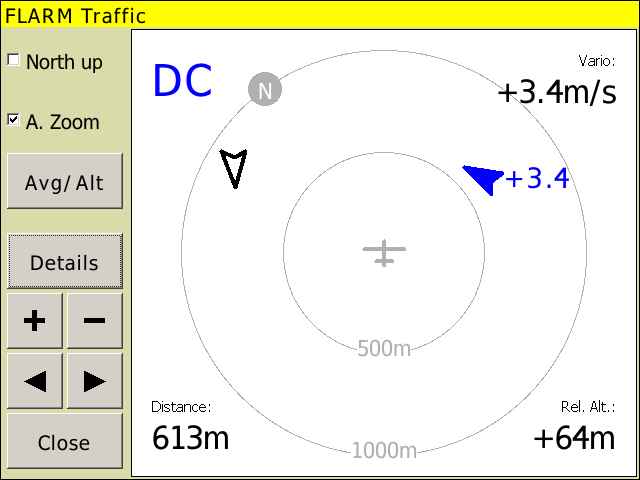
\includegraphics[angle=0,width=0.5\linewidth,keepaspectratio='true']{figures/dialog-flarm1.png}
\end{center}

Somente alguns controles da tela, de cima para baixo:
\begin{description}
\item[Norte acima]  se ativado, a tela será orientada ‘norte acima’, caso contrário a orientação será ‘rota acima’.
\item[A. Zoom]  \gesture{Up - Down} : ajusta o radar automaticamente na tela para que os alvos sejam perfeitamente visíveis.  Se não ativado, a tela terá zoom manual.  O gesto Cima-Baixo ativa o zoom automático.
\item[Avg/Alt]  \gesture{Right - Left} o botão alterna entre o variômetro médio e a altitude mostrada próximo ao alvo.
\item[Detalhes]  \gesture{Down - Right} : através deste botão, é acessado um diálogo separado com todos os detalhes do alvo.
\item[+/-]  \gesture{Up/Down} muda o zoom manualmente do alcance do radar de 500 até 1.000 metros.  O gesto para zoom também se aplica.
\item[$\triangleleft$/$\triangleright$]  \gesture{Left/Right} seleciona entre o alvo anterior e posterior no radar, os gestos funcionam da mesma maneira
\end{description}

\begin{center}
\begin{tabular}{c c}
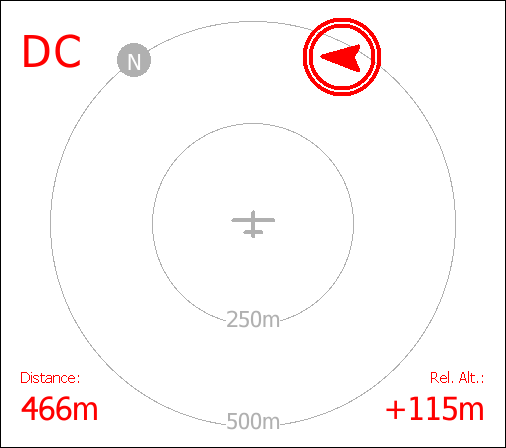
\includegraphics[angle=0,width=0.5\linewidth,keepaspectratio='true']{figures/cut-flarm2.png}&
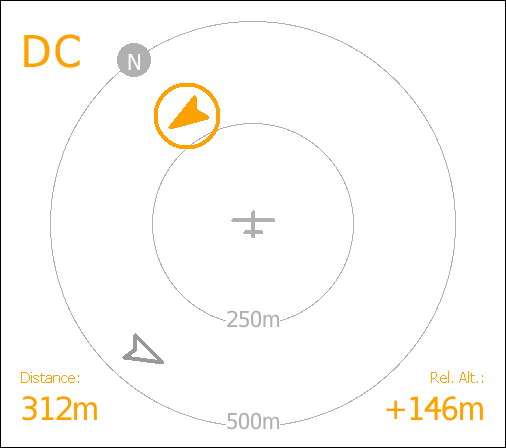
\includegraphics[angle=0,width=0.5\linewidth,keepaspectratio='true']{figures/cut-flarm3.png}\\
\end{tabular}
\end{center}
Estas duas imagens da tela foram tiradas na sequência para demonstrar uma passagem comum de dois planadores equipados com FLARM.  A informação extra é colorida de acordo com os códigos já mencionados.  Nos quatro cantos da tela de radar estão informações adicionais do alvo selecionado:

\begin{description}
\item[Superior esquerdo]  se disponível, o ID FLARM do alvo selecionado.
\item[Superior direito]  variômetro do alvo, derivado das mensagens de altitudes consecutivas.
\item[Inferior esquerdo]  distância ao alvo.
\item[Inferior direito]  a altura relativa do alvo.
\end{description}

Da primeira até a segunda tela do FLARM, se passaram 15 segundos.  O alvo selecionado azul estava subindo a 3,4m/s e sua trajetória não tinha reconhecida como ameaça.  Neste meio tempo, o “DC” virou mais para a esquerda, e se tornou um alerta de ameaça e agora é mostrado em vermelho.  O radar FLARM alterou o zoom de 1.000 para 500 metros.  

\section{Equipe de vôo}\label{sec:team-flying}

O código de vôo é um sistema que permite aos pilotos que voam no mesmo time comunicarem suas posições uns aos outros de uma maneira concisa e precisa.  O princípio do sistema é que cada piloto use seu computador para determinar um código de 5 dígitos que descrevem suas posições relativas a um waypoint comum.  Os pilotos podem chamar uns aos outros reportando estes códigos e entrando com estes códigos no computador permite que o computador localize precisamente seus colegas.

Para usar o código de time, todos os pilotos do time devem selecionar o mesmo waypoint de referência. .  Isto é feito na janela de configuração de código. 
\menulabel{\bmenug{Info 2}\blink\bmenut{Team}{Code}}
O waypoint de referência é definido através do botão “Ajuste WP”.  Selecione um waypoint através da janela e será a referência do time.

Durante o vôo, o piloto pode ler seu próprio código através da janela de código de time, para reportar sua posição ao outro colega do time.  Quando o piloto escuta um código reportado por outro colega, e clica em \button{Set Code} 
para abrir a janela de entrada de texto e permitir a entrada do código do seu colega.
\sketch{figures/dialog-teamcode.png}

Após entrar com o código do seu colega, a distância e a direção são calculadas e atualizadas na janela.  

\subsection*{Procura de Id do FLARM}

XCSoar também suporta códigos de times encriptados através da rede FLARM.  O botão  \button{Flarm Lock} permite que se acesse o banco de dados da rede FLARM, bem como o banco de dados do XCSoar para achar um colega.  Uma simples procura pelo ID de um determinado competidor pode trazer a identidade FLARM.  Selecionando a base de dados desejada dos itens encontrados permitem à você ‘travar’ seu amigo e não sumir.  Veja Seção~\ref{sec:flarm-ident-file} 
para o detalhamento do banco de dados FLARM.

\menulabel{\bmenug{Info 2}\blink\bmenut{FLARM}{Details}}
Uma funcionalidade similar fornece os detalhes na janela FLARM.  Também permite você procurar o ID do competidor na base de dados e mostrar os detalhes.  

\begin{center}
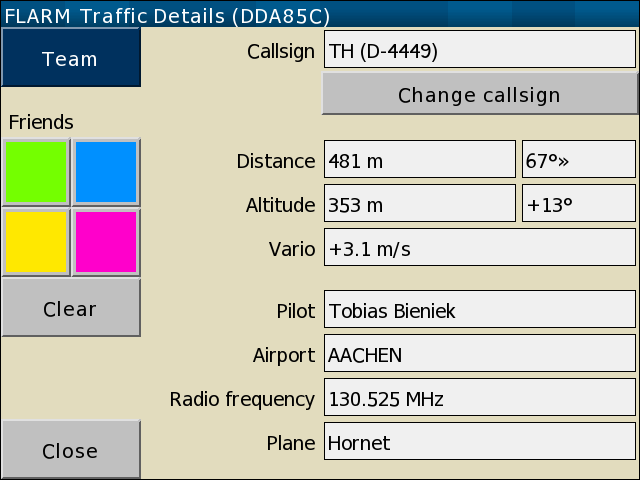
\includegraphics[angle=0,width=0.8\linewidth,keepaspectratio='true']{figures/dialog-flarmdetails.png}
\end{center}


\subsection*{Clique no seu amigo}
Mesmo que o XCSoar possa ‘travar’ somente um colega do time pelo waypoint de referência, pode gerenciar qualquer número de ‘amigos’ quando se sabe seus Ids FLARM.  Há grandes chances do seu amigo não estar registrado em nenhum banco de dados.  Neste caso, você pode voar perto de seu amigo e pegar seus detalhes pelo radar FLARM, escolher a cor e identificar esta resposta no futuro como seu amigo.  


